\section*{Exercise 18 - \textit{Analysis of Temperatures}}

\subsection*{(a)}

First we have to decide whether we can apply a Fourier transformation or Lomb-Scargle periodogram to our data.

In order for a Fourier transformation to be applicable, your data has to be uniformly sampled. If that's not the case, the data needs to be gridded
first. \\

At first, the data we have here looks to be uniformly sampled, but at some point toward the end (from September 18th, 2008, as the exercise sheet so kindly tells us),
the time between measurements decreases from fifteen to ten minutes
(and some data points are just missing entirely or are just broken instead). \\

Such restriction do not apply to the Lomb-Scargle periodogram, which can always be applied to your data.

\subsection*{(b)}

After loading the data from the \texttt{.txt}-file, the code for the Lomb-Scargle periodogram is implemented as seen below.

\begin{lstlisting}[language = Python, caption={Implementation of the Lomb-Scagle periodogram}, label = {list:lombscargle}]
    #0)
    column_names = ["Date", "Time", "Measurement", "Temperature"]
    
    tempdata = pd.read_csv("temperatures_dortmund.csv", names=column_names, sep=",", skiprows=1)
    
    #b)
    Measurement = tempdata["Measurement"].to_numpy()
    Temperature = tempdata["Temperature"].to_numpy()
    
    #we kill everything that is broken
    mask = np.where(Measurement < 2009)
    #Measurement_2 = Measurement(mask)
    M_scarg_1 = Measurement[mask] 
    T_scarg_1 = Temperature[mask]
    #print(len(M_scarg_1))
    #print(len(T_scarg_1))
    mask2 = np.where(~np.isnan(T_scarg_1))
    M_scarg_2 = M_scarg_1[mask2]
    T_scarg_2 = T_scarg_1[mask2]
    freq_max = 400
    
    freq = np.linspace(0.001, freq_max*2*np.pi, 1000) 
    lomb_scarg = lombscargle(np.array(M_scarg_2), np.array(T_scarg_2), freq, normalize=True)
    
\end{lstlisting}

The corresponding plot can be seen in \autoref{fig:lombscarg}

\begin{figure}
    \centering
    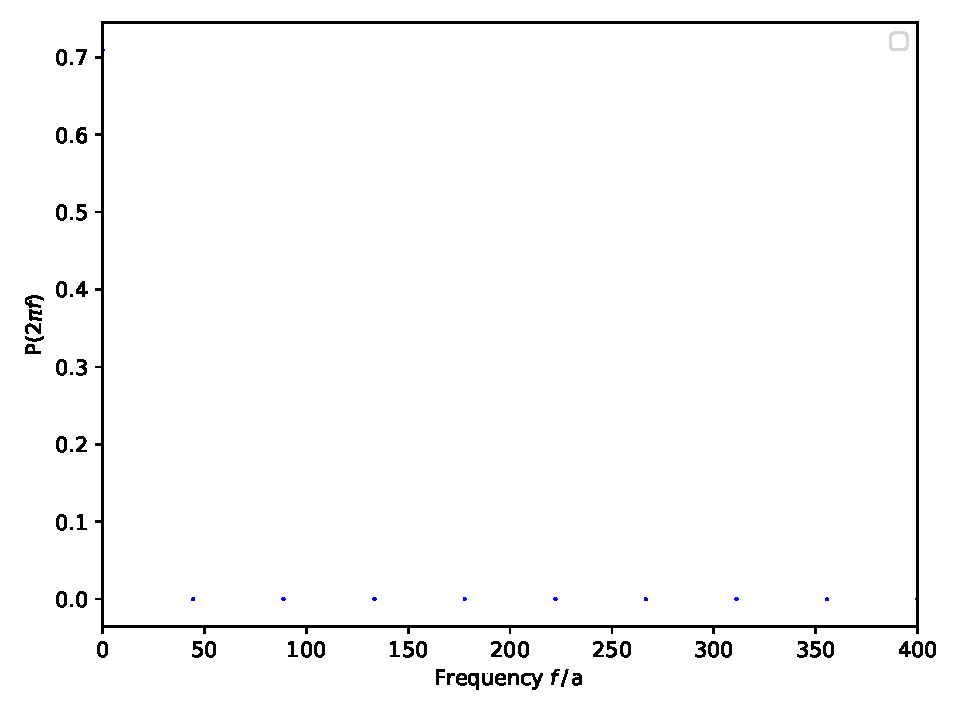
\includegraphics{../lomb_scarg.pdf}
    \caption{Lomb-Scargle periodogram.}
    \label{fig:lombscarg}
\end{figure}
